Using binary to fill in the grid as in the attachment,
a maze is revealed.

\begin{center}
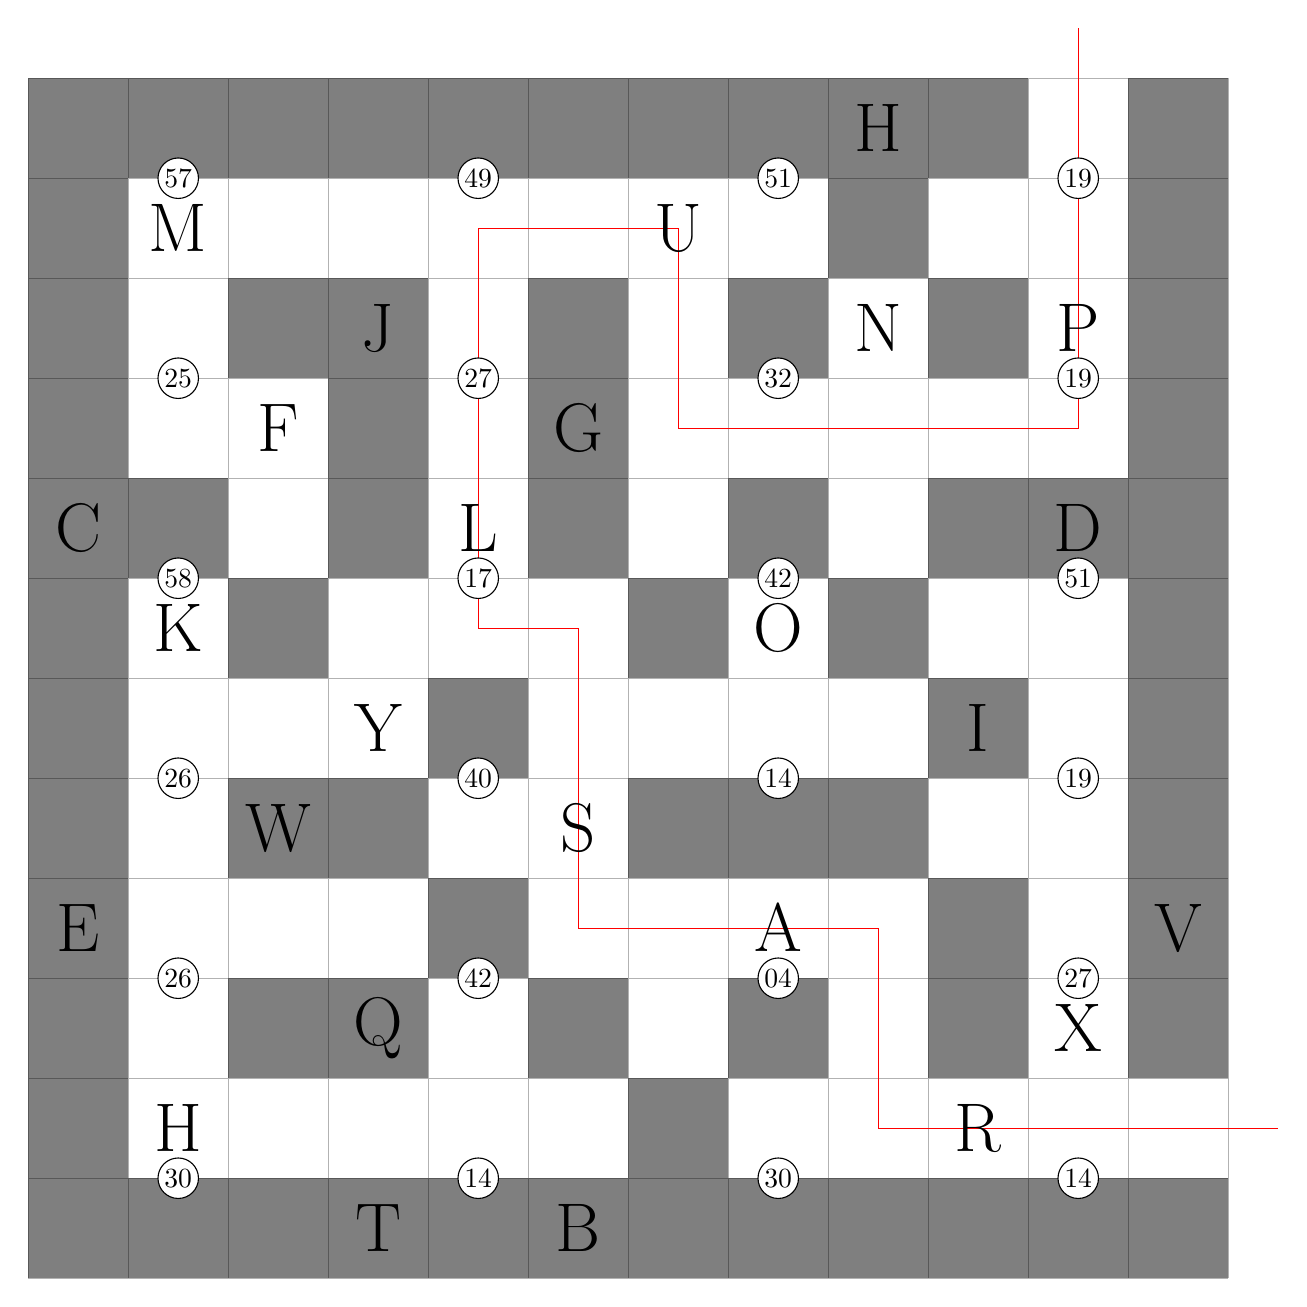
\begin{tikzpicture}[x=0.5in,y=0.5in]
\fill[white] (0,0) rectangle (12,12);
\draw[step=1,black!30] (0,0) grid (12,12);
% solution
\foreach \coor in {
  {(0,0)},
  {(1,0)},
  {(2,0)},
  {(3,0)},
  {(4,0)},
  {(5,0)},
  {(6,0)},
  {(7,0)},
  {(8,0)},
  {(9,0)},
  {(10,0)},
  {(11,0)},
  {(0,1)},
  {(6,1)},
  {(0,2)},
  {(2,2)},
  {(3,2)},
  {(5,2)},
  {(7,2)},
  {(9,2)},
  {(11,2)},
  {(0,3)},
  {(4,3)},
  {(9,3)},
  {(11,3)},
  {(0,4)},
  {(2,4)},
  {(3,4)},
  {(6,4)},
  {(7,4)},
  {(8,4)},
  {(11,4)},
  {(0,5)},
  {(4,5)},
  {(9,5)},
  {(11,5)},
  {(0,6)},
  {(2,6)},
  {(6,6)},
  {(8,6)},
  {(11,6)},
  {(0,7)},
  {(1,7)},
  {(3,7)},
  {(5,7)},
  {(7,7)},
  {(9,7)},
  {(10,7)},
  {(11,7)},
  {(0,8)},
  {(3,8)},
  {(5,8)},
  {(11,8)},
  {(0,9)},
  {(2,9)},
  {(3,9)},
  {(5,9)},
  {(7,9)},
  {(9,9)},
  {(11,9)},
  {(0,10)},
  {(8,10)},
  {(11,10)},
  {(0,11)},
  {(1,11)},
  {(2,11)},
  {(3,11)},
  {(4,11)},
  {(5,11)},
  {(6,11)},
  {(7,11)},
  {(8,11)},
  {(9,11)},
  {(11,11)}
}{ \fill[opacity=0.5] \coor rectangle +(1,1); }
\draw[red] 
  (10.5,12.5) -- 
  (10.5,8.5) --
  (6.5,8.5) --
  (6.5,10.5) --
  (4.5,10.5) --
  (4.5,6.5) --
  (5.5,6.5) --
  (5.5,3.5) --
  (8.5,3.5) --
  (8.5,1.5) --
  (12.5,1.5);
\node at (10.5,9.5) {\Huge P};
\node at (6.5,10.5) {\Huge U};
\node at (4.5,7.5) {\Huge L};
\node at (5.5,4.5) {\Huge S};
\node at (7.5,3.5) {\Huge A};
\node at (9.5,1.5) {\Huge R};
% distractors
\node at (3.5,0.5) {\Huge T};
\node at (5.5,0.5) {\Huge B};
\node at (1.5,1.5) {\Huge H};
\node at (3.5,2.5) {\Huge Q};
\node at (10.5,2.5) {\Huge X};
\node at (0.5,3.5) {\Huge E};
\node at (11.5,3.5) {\Huge V};
\node at (2.5,4.5) {\Huge W};
\node at (3.5,5.5) {\Huge Y};
\node at (9.5,5.5) {\Huge I};
\node at (1.5,6.5) {\Huge K};
\node at (7.5,6.5) {\Huge O};
\node at (0.5,7.5) {\Huge C};
\node at (10.5,7.5) {\Huge D};
\node at (2.5,8.5) {\Huge F};
\node at (5.5,8.5) {\Huge G};
\node at (8.5,9.5) {\Huge N};
\node at (8.5,11.5) {\Huge H};
\node at (3.5,9.5) {\Huge J};
\node at (1.5,10.5) {\Huge M};
%numbers
\node[circle,draw=black,fill=white,inner sep=1pt] at (1.5,11) {57};
\node[circle,draw=black,fill=white,inner sep=1pt] at (4.5,11) {49};
\node[circle,draw=black,fill=white,inner sep=1pt] at (7.5,11) {51};
\node[circle,draw=black,fill=white,inner sep=1pt] at (10.5,11) {19};
\node[circle,draw=black,fill=white,inner sep=1pt] at (1.5,9) {25};
\node[circle,draw=black,fill=white,inner sep=1pt] at (4.5,9) {27};
\node[circle,draw=black,fill=white,inner sep=1pt] at (7.5,9) {32};
\node[circle,draw=black,fill=white,inner sep=1pt] at (10.5,9) {19};
\node[circle,draw=black,fill=white,inner sep=1pt] at (1.5,7) {58};
\node[circle,draw=black,fill=white,inner sep=1pt] at (4.5,7) {17};
\node[circle,draw=black,fill=white,inner sep=1pt] at (7.5,7) {42};
\node[circle,draw=black,fill=white,inner sep=1pt] at (10.5,7) {51};
\node[circle,draw=black,fill=white,inner sep=1pt] at (1.5,5) {26};
\node[circle,draw=black,fill=white,inner sep=1pt] at (4.5,5) {40};
\node[circle,draw=black,fill=white,inner sep=1pt] at (7.5,5) {14};
\node[circle,draw=black,fill=white,inner sep=1pt] at (10.5,5) {19};
\node[circle,draw=black,fill=white,inner sep=1pt] at (1.5,3) {26};
\node[circle,draw=black,fill=white,inner sep=1pt] at (4.5,3) {42};
\node[circle,draw=black,fill=white,inner sep=1pt] at (7.5,3) {04};
\node[circle,draw=black,fill=white,inner sep=1pt] at (10.5,3) {27};
\node[circle,draw=black,fill=white,inner sep=1pt] at (1.5,1) {30};
\node[circle,draw=black,fill=white,inner sep=1pt] at (4.5,1) {14};
\node[circle,draw=black,fill=white,inner sep=1pt] at (7.5,1) {30};
\node[circle,draw=black,fill=white,inner sep=1pt] at (10.5,1) {14};
\end{tikzpicture}
\end{center}

The solution is the letters appearing on the unique solution to the maze:
\texttt{PULSAR}
